\section{Concurrent Data Structures}

In this exercise we are supposed to take a sequential implementation of a 
linked list and make this concurrent. This will demand a sophisticated use of
locks to properly synchronize the list.

\subsection{Coarse Grained Locking using Mutex}

To implement coarse grained locking. A lock on the whole list was implemented.
This means that if any of the methods \textbf{insert}, \textbf{remove} or 
\textbf{count} then the list will become unavailable for other threads while 
this operation runs. This obviously will make it possible to have multiple 
threads operating on the list but it also leaves threads waiting while another 
one operates on it.

To implement this in C++, we updated the sorted list class to have a mutex as a
class variable.

\begin{lstlisting}[language=C++]
template<typename T>
class sorted_list {
	std::mutex li;
	node<T>* first = nullptr;
/* ... class continues ...*/
\end{lstlisting}

And the lock on the list is locked and unlocked like so:

\begin{lstlisting}[language=C++, caption=Coarse-Grained Insert]
    /* insert v into the list */
    void insert(T v) {
        li.lock();
        /* first find position */
        node<T>* pred = nullptr;
        node<T>* succ = first;
        while(succ != nullptr && succ->value < v) {
            pred = succ;
            succ = succ->next;
        }
        
        /* construct new node */
        node<T>* current = new node<T>();
        current->value = v;
    
        /* insert new node between pred and succ */
        current->next = succ;
        if(pred == nullptr) {
            first = current;
        } else {
            pred->next = current;
        }
        li.unlock();
    }
\end{lstlisting}

\begin{figure}
    \centering
    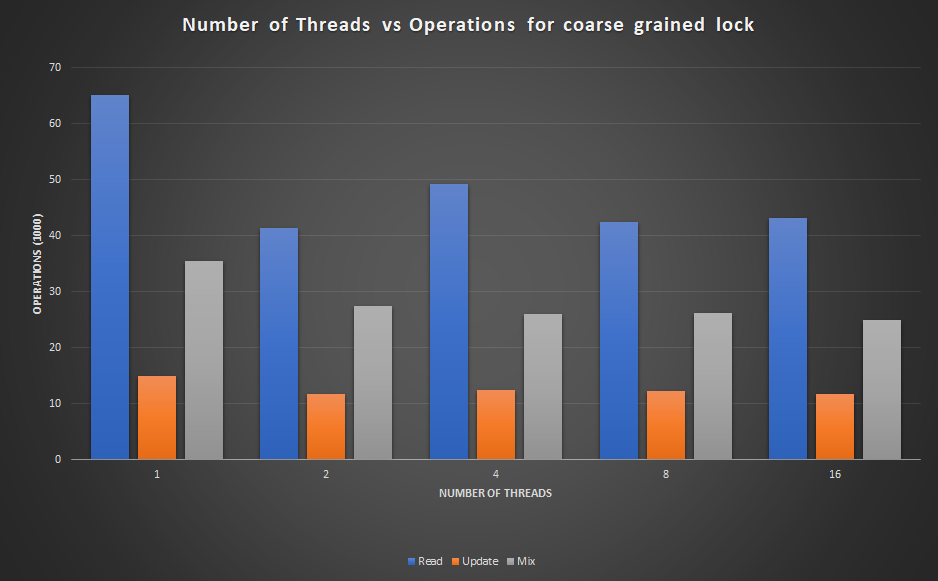
\includegraphics[width=\linewidth]{Figures/coarsegrained.png}
    \caption{Coarse-grained locking with $t \in \{1, 2, 4, 8, 16\}$}
    \label{fig:coarsegrained}
\end{figure}

With a similar implementation for the other methods, the whole method is locked
and the same locked is used for all methods, in essence, the whole list is owned
by a single thread. This implementation works and multiple threads are able to 
run. From simulations we see that the number of operations decrease as more and
more threads are added. This makes sense since there now is introduced overhead
from threads as well as the locking locks out every single thread other than 
the one that is currently in the critical section. This can bee seen in figure
\ref{fig:coarsegrained}.

\subsection{Coarse-grained locking with TATAS}
Here we do the same implementation of locking but the lock we will use is a
Test-And-Test-And-Set (TATAS) lock. This has been implemented by introducing a 
class called TATAS

\begin{lstlisting}[language=C++, caption=TATAS Class]
class tatas {
	private:
		std::atomic<bool> l;

	public:
		tatas() {
			l = false;
		}

		void lock() {
			do {
				while (l) continue;
			} while (l.exchange(1));
			return;
		}

		void unlock() {
			l.exchange(0);
		}
};
\end{lstlisting}

\begin{figure}
    \centering
    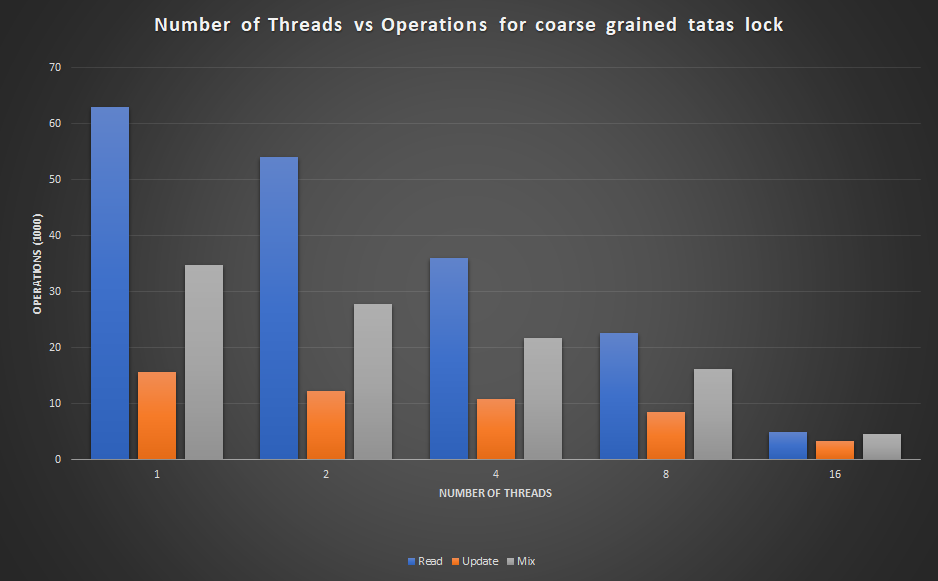
\includegraphics[width=\linewidth]{Figures/coarsegrainedtatas.png}
    \caption{Coarse-grained TATAS locking with $t \in \{1, 2, 4, 8, 16\}$}
    \label{fig:coarsegrainedtatas}
\end{figure}


The implementation for course-grained TATAS just replaces the mutex in the
linked list with this class and calling its lock and unlock method.
The locking works by having a atomic boolean. When a thread calls 'lock'
it continually observes the atomic bool l and when this becomes false. It checks
the value of the boolean with the exchange method. This method returns the value
of the atomic boolean, then tries to change it. So if it has changed to true
in the time before the first check. The do-while loop catches this and it goes 
back. Unlocking is simple and just calls exchange without any further checks.

This implementation works. But when we visualize the performance of this we see
that the performance gets even worse. This is due to the even more extensive 
waiting that threads have to go through in this program as well as the locking
being coarse grained. This is shown in figure \ref{fig:coarsegrainedtatas}.

\section{Fine-grained locking with Mutex}

Our understanding of fine-grained locking is as follows:

\begin{itemize}
	\item To address the challenges seen in the previous sections, another way 
	of calling threads and to synchronies them
	\item Fine-grained has been interpreted by us to mean that each node in the 
	list should have their own locks, and locking nodes that is operated on.
	\item This should allow different threads to concurrently operate on different
	parts of the linked list independently.
	\item This is a non-trivial task since when doing the search through the list.
	The locking and unlocking of threads must be done correctly to ensure that no
	nodes are locked when they should not be.
	\item This is a non-trivial task since our implementation must ensure that
	the data structure remains intact and in order. 
	\item Our idea. When searching through the list, one points to two nodes at 
	a time and update these as one moves through the list. When the node that 
	is last of the two nodes has served its purpose (we no longer need to read
	its data), this should be unlocked. 
	\item When inserting a node. The two nodes that it will be inserted into 
	must be locked.
\end{itemize}

We have tried to do this by introducing mutexes in each node:

\begin{lstlisting}[language=C++, caption=Node with lock]
/* struct for list nodes */
template<typename T>
struct node {
	T value;
	node<T>* next;
	std::mutex l;
};
\end{lstlisting}

And here is how we implemented the insert method:

\begin{lstlisting}
/* insert v into the list */
void insert(T v)
{
	/* first find position */
	node<T> *pred = nullptr;
	l.lock();
	node<T> *succ = first;
	if(succ) succ->l.lock();
	l.unlock();
	/* Check that first is not nullptr*/
	while (succ != nullptr && succ->value < v)
	{
		pred = succ;
		succ->l.unlock();
		succ = succ->next;
		if (succ != nullptr)
		{
			succ->l.lock();
		}
	}

	/* construct new node */
	node<T> *current = new node<T>();
	current->value = v;

	/* insert new node between pred and succ */
	current->next = succ;
	if (pred == nullptr)
	{
		first = current;
	}
	else
	{
		pred->next = current;
	}
	if (succ) succ->l.unlock();
}
\end{lstlisting}

The other methods implementation can be found in the attached code.
Whilst the code compiles and executes successfully with a single thread,
upon introducing >1 thread, data-races were present due to the incorrect order of locking 
and unlocking. 
Due to time limitations we were unable to debug this section further. 
However, based on what was observed in the test with a single thread, the performance of the 
program should increase in a noticeable fashion as the linked list can be interacted with by multiple threads 
simultaneously (provided operations are occurring on different sections of the list)

\section{Fine-grained locking with TATAS}
% TODO - Insert proposed coding implementation here (should be the same as code above except substitute the locks with the TATAS implementation you already wrote)

Similar to our results in the Fine-grained locking with mutex (TODO - INSERT SECTION REFERENCES HERE)
The other methods implementation can be found in the attached code.
And once again, whilst the code compiles and executes successfully with a single thread,
upon introducing >1 thread, data-races were present due to the incorrect order of locking 
and unlocking. 
Due to time limitations we were unable to debug this section further. 
However, based on what was observed in the test with a single thread, and with a knowledge of how TATAS locking functions,
we can assume that the performance would be quicker than all coarse-grained implementations as threads increase, however it would be worse than the mutex lock above.
This is presumed to be due to the extra locks and cache-busts which occur when a lock is released.

\section{Fine-grained locking with scalable queue lock}

% TODO - Insert proposed coding implementation here (should be the same as code above except substitute the locks with the a queue lock implementation from the slides)

Similar to our results in the Fine-grained locking with mutex (TODO - INSERT SECTION REFERENCES HERE) or Fine-grained locking with TATAS (TODO - INSERT SECTION REFERENCES HERE)
The other methods implementation can be found in the attached code.
And once again, whilst the code compiles and executes successfully with a single thread,
upon introducing >1 thread, data-races were present due to the incorrect order of locking 
and unlocking. 
Due to time limitations we were unable to debug this section further. 
However, based on what was observed in the test with a single thread, and with a knowledge of how queue-locks operate, 
we can assume a substantial speed-up as the number of threads increase (superseding all other implementations thus far). 
The cost does occur in the complexity of code written.